\documentclass[leqno]{beamer}
\usepackage[T1]{fontenc}

\usepackage{pgf,pgfpages}
\usepackage{tikz}
\usetikzlibrary{arrows,shapes,backgrounds,calc}

\usepackage{graphicx}
\usepackage{colortbl}
\usepackage{fancybox}
\usepackage{units}

\newcommand{\OK}{{\color{PHDgreen}\ding{52}}}

%% Beamer style.....
\mode<presentation>
{
  \usetheme{PHD}
  \setbeamercovered{transparent}
  \setbeamertemplate{items}[square]
}

% \usefonttheme[onlymath]{serif}

\beamertemplatenavigationsymbolsempty

\defbeamertemplate{enumerate item}{mycircle}
{
  % \usebeamerfont*{item projected}%
  \usebeamercolor[bg]{item projected}%
  \begin{pgfpicture}{0ex}{0ex}{1.5ex}{0ex}
    \pgfcircle[fill]{\pgfpoint{-0.1pt}{.65ex}}{1.1ex}
    \pgfbox[center,base]{\color{PHDyellow}{\insertenumlabel}}
  \end{pgfpicture}%
}
[action]
{\setbeamerfont{item projected}{size=\scriptsize}}
\setbeamertemplate{enumerate item}[mycircle]

% ..............beamer style

\newcommand{\strip}[1]{%
  \begin{flushright}
    \color{PHDgrayC}
    \scriptsize{#1}
  \end{flushright}}

\title[Stable Schemes Non-Hydrostatic Large-Scale]
% [Quasi-Hydrostatic Equations]
{On Stable Schemes for Large-Scale Non-Hydrostatic Boussinesq Equations}
\author[J. R. Rguez. Galv\'an]{%
  { J. Rafael Rodr\'{\i}guez Galv\'an
    \\[0.5em]
    {\small \textit{Workshop: non-hydrostatic effects in oceanography}}
  }}
\date{October 15, 2018}

% XeLaTeX font choosing
% \usepackage{fontspec}%{xltxtra} %fontspec}
% \setsansfont{Fontin Sans}
% \setsansfont{Lato}

% PDFLaTeX font choosing
\usepackage[default, scale=1.0]{lato}
% \usepackage[math, default, scale=0.95]{vollkorn}

% Different math fonts, see http://tug.org/pracjourn/2006-1/hartke/hartke.pdf
% \usepackage{eulervm}
% \usepackage{ccfonts, eulervm}
% \usepackage[math]{kurier}
% \usepackage[math]{anttor}
% \usepackage{pxfonts}
% \usepackage{mathpazo}
% \usepackage{mathpple}
% \usepackage[varg]{txfonts}
% \usepackage{arev}
% \usepackage{fourier}

\usepackage{tabularx}
\usepackage{array, multirow, booktabs, rotating} % booktabs: toprule, midrule...

% Define a special style at begining of sections
\newcommand{\SetEmptyBackground}{
  \setbeamertemplate{background}{}
  \setbeamertemplate{footline}[default]
}
\newcommand{\SetDefaultBackground}{
  \setbeamertemplate{background}
  {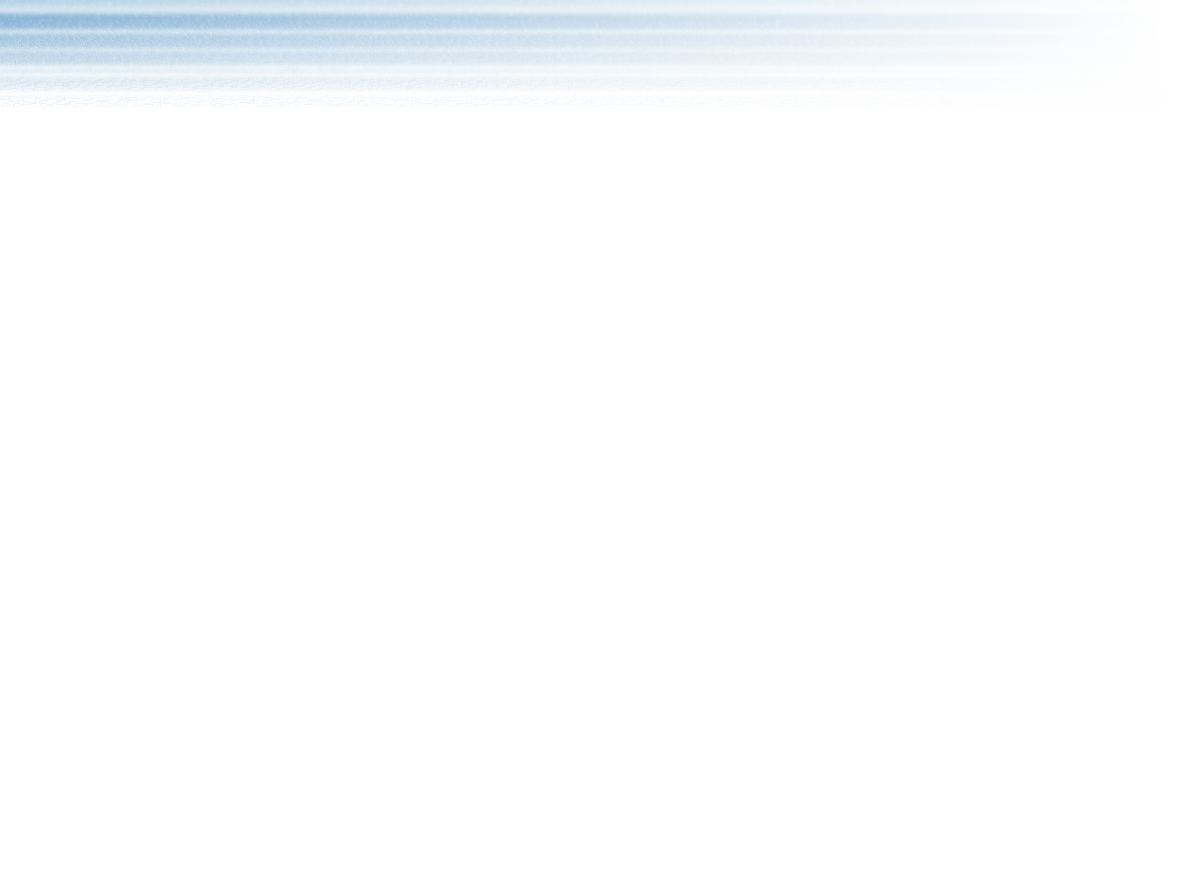
\includegraphics[width=\paperwidth,height=\paperheight]{slide_bg}}
  \setbeamertemplate{footline}[PHDtheme]
}
\newenvironment{sectionframe}{%
  \SetEmptyBackground\begin{frame}
    % \par\noindent\structure{\rule{\linewidth}{1pt}}\par
    % \vskip+0.6em
    \vskip1.6em
    Section \thesection.  \itshape\insertsection
    \vskip-0.7em
    \par\noindent\structure{\rule{\linewidth}{1pt}}\par
  }{%
  \end{frame}\SetDefaultBackground}

\newenvironment{smallblock}[1]{%
  % Block with horizontal top title
  \begin{block}{\small #1}
    \vspace{-0.9\baselineskip}
    \small
  }{\vspace{-1.2\baselineskip}\end{block}}


%%%%%%%%%%%%%%%%%% Vídeo!
% \usepackage{media9}
\usepackage{multimedia}

% PHD specific stuff....
\usepackage{rrgalvan-nonhyd2018}

\newtheorem{remark}{Remark}
% \newtheorem{theorem}{Theorem}

\newcommand{\step}[1]{\par\textbf{Step #1}.}
\newcommand{\substep}[1]{\par\textsf{Step #1}.}

\newcommand{\aniNS}{\emph{(Anis-NStokes)}\xspace}
\newcommand{\hydNS}{\emph{(Hydr-NStokes)}\xspace}
\newcommand{\hydStokes}{\emph{(Hydr-Stokes)}\xspace}
\newcommand\hydStokesDiscr{\ensuremath{\text{\emph{(Hydr-Stokes)}}_h}\xspace}
% ...

% Presentation goodies
\newcommand<>{\myframed}[1]{\alt#2{\tikz[phd] \node[box] {#1};}{{#1}}}
\newcommand<>{\myframedAlert}[1]{\alt#2{\tikz[phdB] \node[boxB] {\color{black}#1};}{{#1}}}
\newcommand<>{\framedmath}[1]{%
  \alt#2{\tikz[phd] \node[box] {\ensuremath{#1}};}{\ensuremath{#1}}}
\newcommand{\framedB}[1]{\tikz[phd] \node[boxB] {#1};}
\newcommand{\framedmathB}[1]{\framedB{\ensuremath{\displaystyle{#1}}}}
\newcommand{\ver}[1]{\footnote{See #1}}
\newcommand{\cita}[1]{{\color{PHDgray}\cite{#1}}}
\newcommand\cellalert[2]{\only<#1>{\cellcolor{PHDyellow}}\alt<#1>{\textbf{#2}}{#2}}
\newcommand{\rowalert}[7]{%
  \cellalert{#1}{#2} & \cellalert{#1}{#3} &
  \cellalert{#1}{#4} & \cellalert{#1}{#5} &
  \cellalert{#1}{#6} & \cellalert{#1}{#7}}

\newcommand{\kk}{\Delta t}
% \usepackage{wasysym}
% %% ,---------------------------------------------------------------------
% %% | Hydrostatic Stokes Stability
% %% `---------------------------------------------------------------------
% \section{Hydrostatic Stokes Stability}
% \include{sec-hydrstokes-stability}

% %% ,---------------------------------------------------------------------
% %% | Stokes with Unequal FE for Velocity
% %% `---------------------------------------------------------------------
% \section{Stokes with Unequal FE for Velocity}

%% ,---------------------------------------------------------------------
%% | Hydrostatic Stable FE combinations}
%% `---------------------------------------------------------------------
% \newcommand{\good}{{\color{PHDgreen}$\CIRCLE$}} %\blacksmiley
% \newcommand{\bad}{{\color{PHDred}$\CIRCLE$}}
\usepackage{pifont}
\newcommand{\good}{{\color{PHDgreen}\ding{52}}}
\newcommand{\bad}{{\color{PHDred}\ding{56}}}
\newcommand{\exclamation}{{\large\color{PHDred}{\textbf{\itshape !}}}}
\newcommand{\question}{{\large\color{PHDred}{\textbf{\itshape ?}}}}
\newcommand\colorUnderLine[2][PHDyellow]{\color{#1}\underline{{\color{black}#2}}\color{black}\xspace}
\newcommand\gris{\color{PHDgray}}
\newcommand\amarillo{\color{PHDyellow}}

\newcommand{\nonFundHipo}{
  \begin{rotate}{30}
    \structure{
      \ovalbox{\tiny\bf%
        \begin{tabular}{@{}c@{}} Non-fundamental
          \\
          hypothesis!
        \end{tabular}
      }
    }
  \end{rotate}
}

\newenvironment{BoxWithVerticalLabel}[2]{%
%  \begin{tabular}{@{\quad}r@{ }l@{}}
  \mbox{}\quad
  \begin{rotate}{90}
    \color{black}\small\fbox{#1}
  \end{rotate}}%&}
{}

% Video playing
% Commands with two or more optional arguments
% (see http://tex.stackexchange.com/questions/29973/more-than-one-optional-argument-for-newcommand)
\usepackage{xparse} % From future LaTeX 3
\DeclareDocumentCommand{\PlayVideoWithLabelAutostart}{%
  O{0.5\linewidth} O{0.5\linewidth}  O{} m }{%
  % #1: width of video box
  % #2: height of video box
  % #3: Label
  % #4: Video file
  \begin{BoxWithVerticalLabel}{#3}{#1}
    \href{run:#4?autostart}{\rule{#1}{#2}}
  \end{BoxWithVerticalLabel}}

\DeclareDocumentCommand{\PlayVideoWithNoLabelAutostart}{%
  O{0.5\linewidth} O{0.5\linewidth} m }{%
  \href{run:#3?autostart}{\rule{#1}{#2}}}

\DeclareDocumentCommand{\PlayVideoNOAutoStart}{%
  O{0.5\linewidth} O{1.0} O{} m }{%
  \href{run:#3}{\rule{#1}{#2}}}

\DeclareDocumentCommand{\PlayVideoWithLabelNOAutostart}{%
  O{0.5\linewidth} O{1.0} O{} m }{%
  \begin{BoxWithVerticalLabel}{#3}{#1}
    \href{run:#4}{\rule{#1}{#2}}
  \end{BoxWithVerticalLabel}}

\DeclareDocumentCommand{\PlayVideoWithLabel}{%
  O{0.5\linewidth} O{1.0}  O{} m }{\PlayVideoWithLabelAutostart[#1][#2][#3]{#4}}

\setcounter{tocdepth}{1}


%
% Bibliography
%
% \usepackage{natbib}

% To list each bibliographic entry in a line
\setbeamertemplate{bibliography entry title}{}
\setbeamertemplate{bibliography entry location}{}
\setbeamertemplate{bibliography entry note}{}

% \includeonly{
% sec-intro,
% sec-hydrstokes-stability,
% sec-stokes,
% sec-hydrstokes-tests,
% sec-v-stabilized,
% sec-vardens-time
% }

%   \includeonly{sec-stokes}
%   \includeonly{sec-hydrstokes-tests}
%   \includeonly{sec-v-stabilized}
%   \includeonly{sec-vardens-time}

%   ... end of preamble.

\AtBeginSection{\frame{\sectionpage}}

%   ======================================================================
\begin{document}
% ======================================================================

% Tikz style and beamer template ------->>>
\tikzstyle{every picture}+=[remember picture]
\tikzstyle{na} = [baseline=-.5ex]
\tikzstyle{phd} = [baseline=-.6ex,
box/.style={rectangle, draw=PHDblueC, thick, fill=PHDblueA,
  align=center, rounded corners, minimum height=1.6em},
boxB/.style={rectangle, draw=PHDredA, thick, fill=PHDblueA,
  align=center, rounded corners, minimum height=1.6em}]
\tikzstyle{phdB} = [baseline=-.7ex,
box/.style={rectangle, draw=PHDblueC, thick, fill=PHDblueA,
  align=center, rounded corners, minimum height=1.6em},
boxB/.style={rectangle, draw=PHDredA, thick, fill=PHDblueA,
  align=center, rounded corners, minimum height=1.6em}]
\tikzstyle{myarrow} = [->,>=latex, PHDredA, shorten >=4pt,
opacity=.6, line width=0.6mm]
\tikzstyle{myarrow2} = [->,>=latex, PHDblueC, shorten >=4pt, opacity=.2, line width=0.4mm]
\tikzstyle{myarrow3} = [
opacity=.7,
% >=triangle 60,              % Nice arrows; your taste may be different
node distance=6mm and 60mm, % Global setup of box spacing
every join/.style={norm},   % Default linetype for connecting
% boxes
line width=0.6mm,
PHDredA,
->
]
\setbeamertemplate{background}
{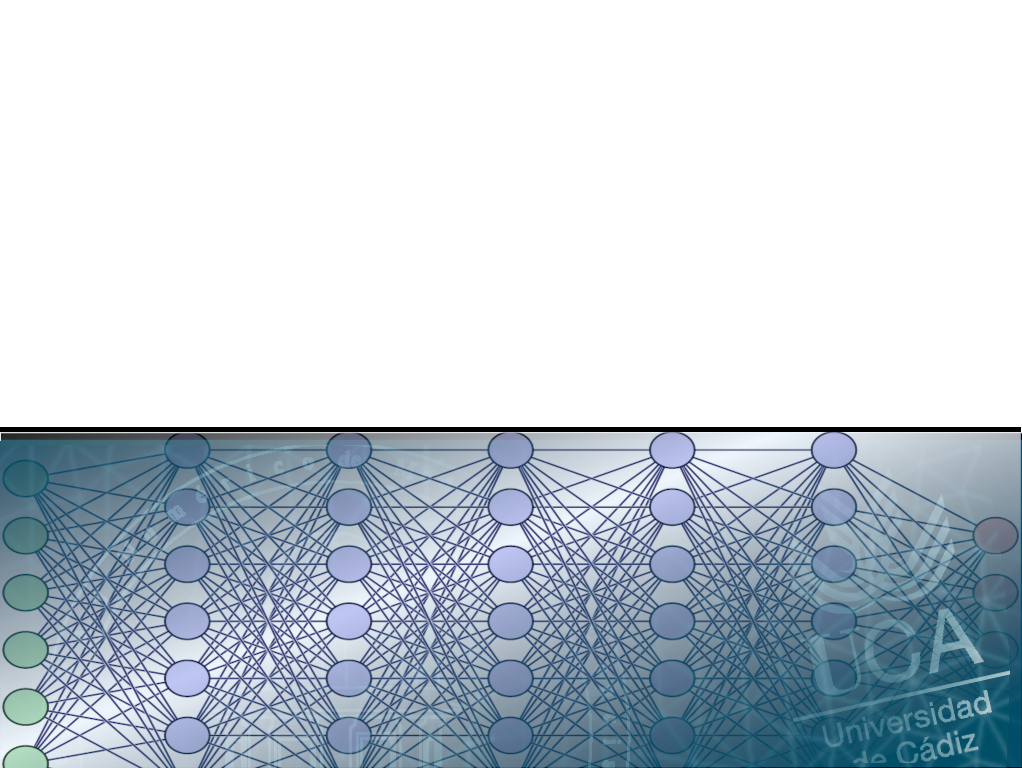
\includegraphics[width=\paperwidth,height=\paperheight]{frontpage_bg}}
\setbeamertemplate{footline}[default]
% <<<-------


% Write custom titlepage ------->>>
\begin{frame}
  \titlepage
  \vspace{5cm}
\end{frame}

% Set the background for the rest of the slides.
% \setbeamertemplate{background}
% {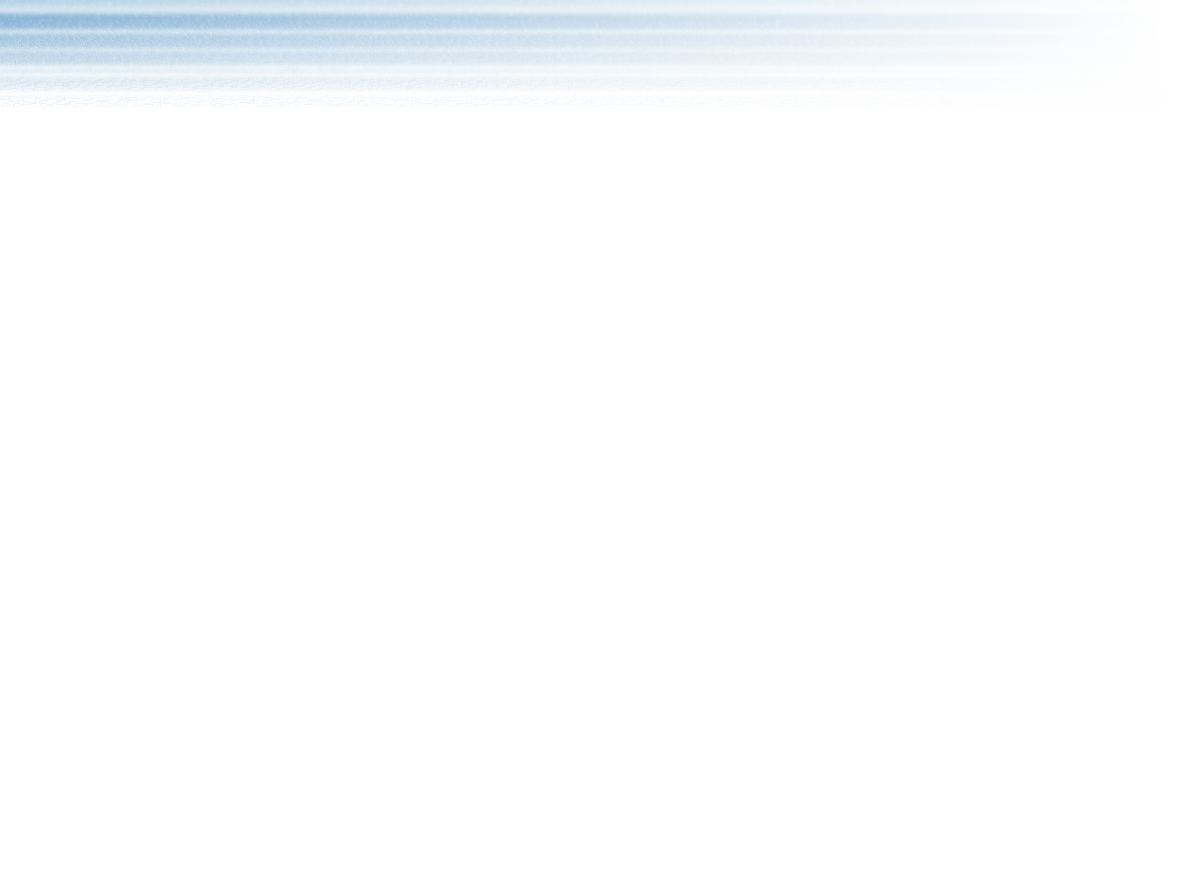
\includegraphics[width=\paperwidth,height=\paperheight]{slide_bg}}
% Set empty background
\setbeamertemplate{background}{}



% Write all of the slides..........
\begin{frame}{Outline}
  \tableofcontents
\end{frame}

% Start inserting infoline at the end
\setbeamertemplate{footline}[PHDtheme]
% <<<-------

\newcommand{\imgdir}{Undefined, use renewcommand!}
\renewcommand{\ISph}{\ensuremath{(IS)^\PP_h}\xspace}
\renewcommand{\ISvh}{\ensuremath{(IS)^\VV_h}\xspace}

%% ,---------------------------------------------------------------------
%% | Introduction
%% `---------------------------------------------------------------------
\section{Introduction}
\label{sec:introduction}


% \begin{frame}
%   % ----------------------------------------------------------------------
%   \frametitle{We present...}
%   \onslide<1->\ovalbox{
%     \begin{tabular}{@{}rl@{}}
%       New \textbf{FE schemes} \scriptsize for
%       &
%         \begin{tabular}{@{}r@{}}
%           \Large \textbf{\textit{Hydrostatic Navier-Stokes}} \scriptsize Equations \\
%           \scriptsize (or {\large\textrm{Primitive Equations}} of the \large\textrm{Ocean})
%         \end{tabular}
%     \end{tabular}}
%   \dotfill\vfill\dotfill
%   \onslide<2->
%   \ovalbox{
%     \begin{tabular}{@{}rl@{}}
%       \scriptsize emphasizing
%       &
%         $\left\{
%         \begin{tabular}{@{}l@{}}
%           \scriptsize use in \Large\textbf{\textit{unstructured FE meshes}},
%           \\
%           \textbf{no} \scriptsize need of \Large\textbf{\textit{vertical integrals}},
%           \\
%           \scriptsize \textbf{\textit{easy implementation}}
%           \tiny (even \textit{non-hydrostatic}. \textit{variable-density} cases).
%         \end{tabular}
%       \right.
%       $
%     \end{tabular}}
%   % \dotfill\hspace{-1ex}\dotfill
%   \vfill\vfill
%   \onslide<3->
%   \ovalbox{
%     \begin{tabular}{@{}rl@{}}
%       \small
%       \begin{tabular}{@{}l@{}}
%         Idea: \normalsize\textbf{\textit{stabilization}} \\ \tiny of vertical velocity makes possible
%       \end{tabular}
%    &
%      $\left\{
%      \begin{tabular}{@{}l@{}}
%        \small to avoid \textbf{``hydrostatic'' inf-sup condition,}
%        \\\noalign{\smallskip}
%        \small to use standard {\large\textit{\textbf{Stokes FE}}} (e.g \P2-\P1)
%      \end{tabular}
%       \right.
%       $
%     \end{tabular}}
%   \small
%   \dotfill\vfill\dotfill
%   \onslide<3->
%   \ovalbox{optimal error order}\dotfill
%   \ovalbox{\scriptsize even for $\dz\pp$\quad \scriptsize(\P{1,b}-\P1, adequate reformulation).}
%   % \dotfill\vfill\dotfill
%   % \ovalbox{numerical experiments.%  support $\left\{
%   %   % \begin{tabular}{l}
%   %       %   theoretical resulsts \\ ease of use our schemes.
%   %       % \end{tabular}
%   %       % \right.$
%   % }
% \end{frame}

\begin{frame}{\alert{Large Scale} Ocean Equations}
  % ----------------------------------------------------------------------
  \begin{itemize}\itemsep1.5em
  \item<1-> \structure{The ocean:} \scriptsize A slightly compressible
    fluid endowed with Coriolis and buoyancy forces % and a set of
    % \normalsize conservation laws from Physics
  \item \structure{Fundamental \textbf{hypothesis}} considered \scriptsize{(for \textit{simplifying} physical laws)}:
    % \vspace{-1em}
    \begin{columns}
      \column{0.05\linewidth}
      \column{0.41\linewidth}
      \begin{enumerate}\itemsep1.5em
      \item<2-> {\small Boussinesq} \scriptsize{hypothesis}
        \tikz[na] \coordinate(Lboussinesq);
        \hfill
        \tikz[na] \coordinate(Rboussinesq);
        % \item<4-> Cartesian coordinates
        %   \tikz[na] \coordinate(LbetaPlane);
        %   \hfill
        %   \tikz[na] \coordinate(RbetaPlane);
      \item<3-> {\small Thin aspect ratio}
        \tikz[na] \coordinate(LverticalScaling);
        \hfill
        \tikz[na] \coordinate(RverticalScaling);
      \end{enumerate}
      \column{0.54\linewidth}
      \begin{overprint}
        \onslide<2>\vspace{\baselineskip}
        \begin{block}{Boussinesq Hypothesis}
          \begin{itemize}
            % \item \textit{Density} does not depart from a \textit{mean reference value},
            %   $\rho_\star>0$
          \item \textbf{Density} is a \structure{\textit{constant}} $\rho_\star$
            \structure{\textit{except in buoyancy}} terms.
          \end{itemize}
        \end{block}
        % \onslide<4>\vspace{3\baselineskip}
        % \begin{block}{Cartesian Coordinates}
        %   Although spherical coordinates are best suited for large
        %   scale earth, they require only the proper handling of some
        %   terms.
        % \end{block}
        \onslide<3>
        \begin{block}{Thin aspect ratio}
          \begin{itemize}\itemsep0.5em
          \item \alert{Anisotropic} (flat) \textbf{domain}
          \begin{equation*}
            \framedmath{\displaystyle\varepsilon = \frac{\text{\textit{vertical}
                  \scriptsize scales}}{\text{\textit{horizontal} \scriptsize scales}}}~
            \begin{tabular}[t]{l} is \large\alert{\textbf{small}} \\[-0.2ex]
              \tiny ~ $10^{-3}$, $10^{-4}$\end{tabular}
          \end{equation*}
          {\tiny {\color{gray}E.g. Mediterranean and North Atlantic: $\varepsilon\simeq 10^{-4}$}}
          \item Then the problem is
            \alert{rescaled}:
            \par
            {\tiny \myframed{Anisotropic domain} $\rightarrow$ \myframed{Isotropic domain}}
          \end{itemize}
        \end{block}
      \end{overprint}
    \end{columns}
  \end{itemize}

  \begin{tikzpicture}[overlay]
    % \draw<2> [thin, red,opacity=.8, fill=red,fill opacity=0.3](stone) circle (4pt);
    % \path<3>[->,>=latex, PHDredA, shorten >=4pt, opacity=.6]
    % (Lboussinesq) edge [out=0, in=130] (Rboussinesq);
    \draw<2>[->, PHDblue, ultra thick, opacity=.8] (Lboussinesq) -- (Rboussinesq);
    % \draw<4>[->, PHDblue, ultra thick, opacity=.8] (LbetaPlane) -- (RbetaPlane);
    \draw<3>[->, PHDblue, ultra thick, opacity=.8] (LverticalScaling) -- (RverticalScaling);
  \end{tikzpicture}
\end{frame}


\begin{frame}{The adimensional domain}
  % \vspace*{0.5em}

  \begin{itemize}\setlength{\itemsep}{1.5em}
  \item After \textbf{vertical scaling}, we obtain an
    \alert{\textbf{isotropic domain}} $\Omega\subset\Rset^3$:
    \begin{tabular}{p{0.37\textwidth} p{0.62\textwidth}}
        \vspace{0pt} 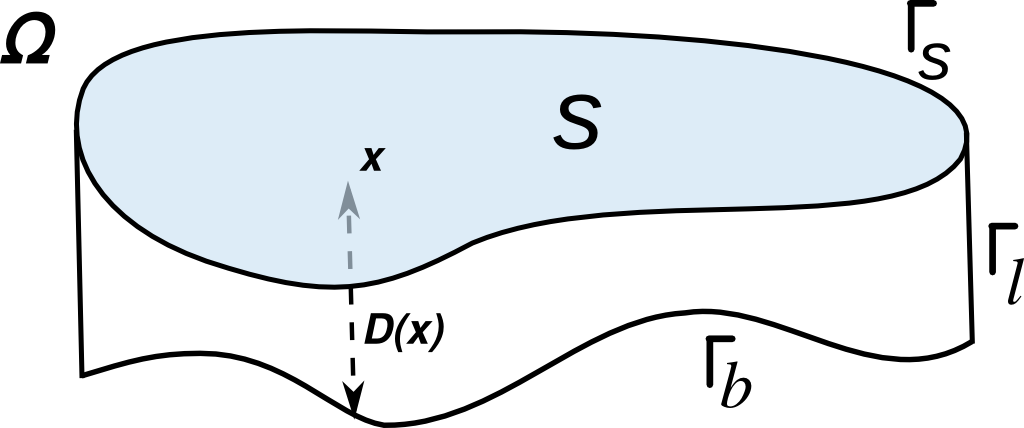
\includegraphics[width=0.37\textwidth, height=4.5\baselineskip]{img/domain}
      &
      \vspace{1.5em}
      \quad
      $\displaystyle \varepsilon =
      \frac{\text{\textit{vertical}
      \scriptsize scales}}{\text{\textit{horizontal} \scriptsize scales}}
      \sim 1$
    \end{tabular}
    % \begin{equation*}
    %   \raggedbottom
    %   \frac{\text{\textit{vertical}
    %   \scriptsize scales}}{\text{\textit{horizontal} \scriptsize scales}}
    %   \sim 1
    %   \qquad
    %   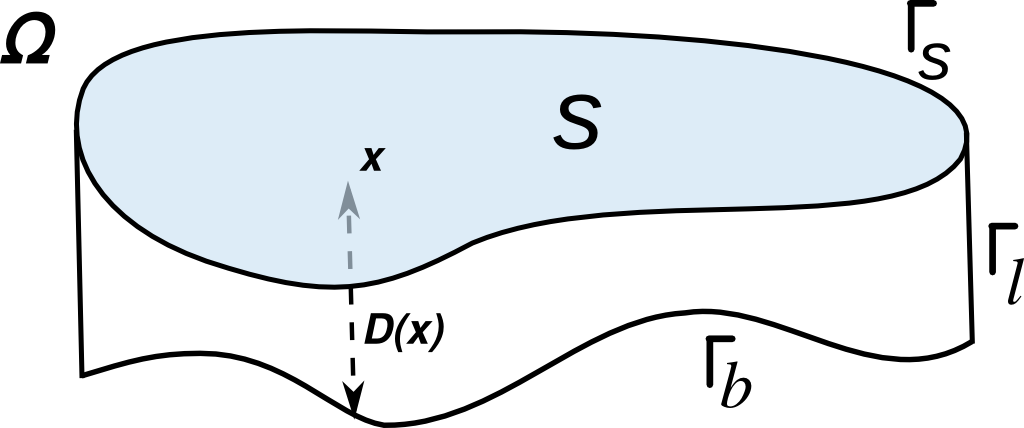
\includegraphics[width=0.35\textwidth, height=4.2\baselineskip]{img/domain}
    % \end{equation*}
    % \vfill
    % \scriptsize Specifically
    % $$
    % \domain = \bigl\{ (\xx,z)\in \Rset^{3} \ /\ \xx=(x,y)\in\surface,\
    % -D(\xx)< z < 0 \bigr\},
    % $$
    % where $\surface\subset\Rset^{2}$ is the surface domain and
    % $D:\overline\surface \to \Rset_{+}$ a depth function

  \item \scriptsize Cartesian coordinates and
    \normalsize \alert{\textbf{rigid lid hypothesis}} {\scriptsize (flat surface)}.
    \begin{quote}
      \scriptsize Also \normalsize \textit{free surface} \scriptsize models might be
      handled by our schemes.\
      \nonFundHipo
    \end{quote}

  \item Vertical scaling the domain $\Rightarrow$ Vertical \alert{scaling} the \alert{equations...}
  \end{itemize}
\end{frame}


\begin{frame}{Large-Scale Boussinesq Equations (variable density)}
  % ----------------------------------------------------------------------
  % \vspace{-0.2em}
  \note{Comment briefly the main difficulties of Navier-Stokes equations}
  \begin{overprint}
    \onslide<1>
    \alert{\textbf{Anisotropic equations}}
    \tikz[na] \coordinate(LaspectRatio);
    % \onslide<2>
    % \alert{Coriolis} force
    % \tikz[na] \coordinate(Lcoriolis);
    \onslide<2>
    \alert{Variable \textbf{density}}~
    \tikz[na] \coordinate(Lcoupling);
    \hfill (coupling temperature and density)
  \end{overprint}
  \begin{block}{\small Conservation of momentum and continuity}
    \vspace{-0.66\baselineskip}
    \begin{align*}
      \dt \uu + \uu\cdot\gradx\uu + \vv\,\dz\uu  - \Delta_\visc\uu
      + \frac 1 \rho_\star \gradx \pp=
      \fU;
      \\
      \tikz[na] \coordinate(RaspectRatio);
      \framedmath<1>{ \varepsilon^2 \Big( \dt \vv + \uu\cdot\gradx\vv +
      \vv\,\dz\vv - \Delta_\visc\vv \Big) }
      \displaystyle
      + \frac 1 \rho_\star \dz \pp +
      \frac{
      \tikz[na] \coordinate(RcouplingA);
      \framedmath<2>{\rho}\,\gravity}{\rho_\star} =
      0\hskip+0.5em
      \\[-0.2em]
      \div\uu + \dz\vv = 0\hskip+0.5em
    \end{align*}
    \vspace{-1.4\baselineskip}
  \end{block}
  \uncover<2>{
    \begin{block}{\small Convection-diffusion of \textit{temperature} and
        \textit{salinity} + state equation (density)}
      \vspace{-0.66\baselineskip}
      \begin{align*}
        \dt \Te  + (\uu \cdot \gradx) \Te + (\vv\cdot\dz) \Te  - \nu_\Te\Delta \Te &= \fT
        \\[0.3em]
        \dt \Sa  + (\uu \cdot \gradx) \Sa + (\vv\cdot\dz) \Sa -
        \nu_\Sa\Delta \Sa &= \fS
        \\[0.3em]
        \tikz[na] \coordinate(RcouplingB);
        \framedmath<2>{\rho} = \rho_\star\big(1-\beta_\Te(\Te-\Te_\star) + \beta_\Sa(\Sa&-\Sa_\star)\big)
      \end{align*}
      \vspace{-1.4\baselineskip}
      % \item Equation of state (dependence of density in terms of
      %   temperature and salinity)
      %   where $\Te_\star$ and $\Sa_\star$ are given reference values.
    \end{block}
  }
  \tikzstyle{RaspectRatio} = [draw, circle, minimum size=.5cm, node
  distance=1.75cm]
  \tikzstyle{redcircle} = [draw, circle, color=PHDredA, node distance=3cm,
  minimum height=2em]

  \begin{tikzpicture}[overlay]
    \path<1>[myarrow]
    (LaspectRatio) edge [out=320, in=130] (RaspectRatio);
    \path<2>[myarrow]
    (Lcoupling) edge [out=0, in=135] (RcouplingA);
    \path<2>[myarrow]
    (Lcoupling) edge [out=0, in=135] (RcouplingB);
  \end{tikzpicture}
\end{frame}

\section{Constant Density Case}

\begin{frame}{Constant Density Non-Hydrostatic Equations}
  % ----------------------------------------------------------------------
  \begin{itemize}\setlength{\itemsep}{1.0em}
  \item \emph{Temporarily}, we introduce the \alert{\textbf{constant density hypothesis}}
  \item Hence we focus on momentum equations:
  \end{itemize}
  \begin{block}{\scriptsize Quasi-Hydrostatic or
      \normalsize\textbf{\ovalbox{Anisotropic} Navier-Stokes}
      \scriptsize equations}
    \begin{align*}
      \dt \uu + \uu\cdot\gradx\uu + \vv\,\dz\uu - \Delta_\visc\uu +
      % \frac 1 \rho_\star
      \gradx \pp= \fU
      \\
      \varepsilon^2 \Big( \dt \vv + \uu\cdot\gradx\vv + \vv\,\dz\vv -
      \Delta_\visc\vv \Big)
      +
      \dz \pp = 0
      \\
      \div\uu + \dz\vv = 0
    \end{align*}
    \vspace{-1.4\baselineskip}
  \end{block}
  \scriptsize
  {\color{gray}
  \begin{align*}
    \text{With adequate boundary conditions, e.g.} \quad
    \nu_z\dz\uu|_{\surfaceBoundary} &= \gs, \quad
                                      \uu|_{\bottomBoundary\cup\talusBoundary}=0 ,
    \\
    % \intertext{adherence on bottom and talus:}
    \vv|_{\bottomBoundary} &=0, \quad
                             \vv|_{\surfaceBoundary} =0, \quad
                             % \intertext{and slip condition on talus:}
                             \gradx\vv \cdot \mathbf{n_x}|_\talusBoundary =0.
  \end{align*}
  }

\end{frame}


\begin{frame}{Hydrostatic Navier-Stokes (or Primitive) Equations}
  % ------------------------------------------------------------
  \begin{small}
    Simplification \framedmath{\varepsilon=0} leads to...
  \end{small}
  \begin{block}{\normalsize\textbf{\ovalbox{Hydrostatic Navier-Stokes}} \scriptsize or Primitive Equations}
    \vspace*{-1em}
    \begin{align*}
      \dt\uu + (\uu\cdot\gradx)\uu +\vv\dz \uu
      - \Delta_\visc\uu + \gradx\pp &= \ff \ \In\domain,
      \\
      \dz\pp & = 0 \ \In\domain,
      \\
      \divx\uu +  \dz\vv &= 0 \ \In\domain.
    \end{align*}
  \end{block}
  \vfill
  \ovalbox{\scriptsize
    % \begin{tabular}{r}
      Usual approach:
      % \\
      % (theoretical and numerical)...
    % \end{tabular}
  }
  \dotfill
  \ovalbox{
    \begin{tabular}{l}
      \small ...$z$--integration $\Rightarrow$ equivalent
      \\ \large\textbf{\alert{differential-integral}}
      \small problem.
    \end{tabular}
  }
  \dotfill\vfill\dotfill
  \ovalbox{
    Pros and cons
  }
  \dotfill
  \ovalbox{%
    \scriptsize
    \begin{tabular}{r}
      \textbf{difficult} \\ handling \\ of
    \end{tabular}
    \small
    $\left\{
      \begin{tabular}{@{}l@{}}
        % standard FE {\scriptsize (unstructured meshes)}, \\
        \alert{non-hydrostatic} case, \\
        variable density,\\
        \scriptsize non-sidewall boundary
      \end{tabular}
    \right.$
  }
\end{frame}

\begin{frame}{Targets}
  \begin{itemize}\itemsep1.3em
  \item \structure{\textbf{Our aim}}:
    \par\bigskip
    \scriptsize Handle both \normalsize $\left\{
      \begin{tabular}{@{}l@{}}
        \textbf{Hydrostatic} and \\[0.3em]
        \textbf{Anisotropic} (non-hidrostatic)
      \end{tabular}
    \right.$
    \par\medskip\hfill{\scriptsize ...equations} \textbf{like standard Navier-Stokes}
  \item That means: developing an \alert{unified framework} for handling
    \textbf{anisotropic} equations for \alert{any $\varepsilon\ge 0$}
  \item \structure{\textbf{Not straightforward}}:
    \begin{itemize}\itemsep0.7em
    \item Usual Navier-Stokes difficulties \llaveizq{Mixed problem
        \\[0.3em]
        Loss of elipticity when Re$\to +\infty$}
    \item \alert{\large New loss of elipticity when $\varepsilon\to 0$}
    \end{itemize}
  \end{itemize}
\end{frame}

\begin{frame}{Usual FE are not valid for \aniNS when $\varepsilon\to 0$}
  \vspace*{0.25em}
  \begin{itemize}\itemsep0.33em
  \item Example: \P2-\P1 cavity test when $\varepsilon\to 0$
    \hfill{\small $\varepsilon=1,...,10^{-5}$)}
  \item \myframed{\textbf{Instabilities} when $\varepsilon\lesssim
      10^{-3}$ \hspace{5.2em}..due to vertical velocity}
    \note{Instabilities are due to anisotropy in domain (or in equations)}
  \end{itemize}
  \vspace*{0.25em}
  \begin{columns}
    ~\hspace{2em}
    \column{0.6\linewidth}
    \PlayVideoWithLabel[0.9\linewidth][0.85\linewidth][Streamlines]{%
      video/eps-to-zero-P2-P1-streamlines-20s.avi}
    \column{0.4\linewidth}
    \centering\PlayVideoWithLabel[0.62\linewidth][0.62\linewidth][Horizontal
    \ $\uu$]{%
      video/eps-to-zero-P2-P1-u-20s.avi}
    \\[0.3em]
%    \par\vskip-0.62em
    \centering\PlayVideoWithLabel[0.62\linewidth][0.62\linewidth][Vertical
    \ $\vv$]{%
      video/eps-to-zero-P2-P1-v-20s.avi}
    \end{columns}
  % \begin{center}
  %   \PlayVideoWithLabel[0.5\linewidth][0.5\linewidth][Streamlines]
  %   {video/eps-to-zero-P2-P1-streamlines.avi}
  % \end{center}
  \begin{flushright}
  \end{flushright}
\end{frame}


\begin{frame}{A completely (mixed) differential formulation}
  \vspace{-0.3em}
  \begin{itemize}\itemsep1em
  \item {\structure{\textbf{Steady linear}} variational formulation:} \hfil
    {\color{gray}\scriptsize find
      $(\uu,\vv,\pp)\in\UU\times\VV\times\PP$ such that}
    \begin{block}{}\vspace{-1.5em}
      \begin{alignat*}{2}
        \nu (\grad\uu,\grad\bu) - (\pp, \divx\bu) &=
        \langle\ff,\bu\rangle &\quad \forall\bu\in\UU,
        \\
        \varepsilon (\grad\uu,\grad\bv) - (\pp,\dz\bv) & = 0 & \quad \forall\bv\in\VV,
        \\
        (\div(\uu,\vv),\bp) &= 0 &\quad \forall\bp\in\PP,
      \end{alignat*}
    \end{block}
    {\scriptsize \color{gray}where $(\cdot,\cdot)$ is the $L^2(\Omega)$ scalar product}
    \vspace{-0.5em}
  \item {\scriptsize $\varepsilon\to 0$, we focus on the \textbf{less
      favorable case: hydrostatic equations} ($\varepsilon=0$)}
    \begin{block}{}\vspace{-1.5em}
      \begin{alignat*}{2}
        \nu (\grad\uu,\grad\bu) - (\pp, \divx\bu) &=
        \langle\ff,\bu\rangle &\quad \forall\bu\in\UU,
        \\
        (\pp,\dz\bv) & = 0 & \quad \forall\bv\in\VV,
        \\
        (\div(\uu,\vv),\bp) &= 0 &\quad \forall\bp\in\PP,
      \end{alignat*}
    \end{block}
    \vspace{-1.5em}
    \pause
    \begin{align*}
      % \UU&=\Uspace=\big\{\uu\in H^1(\Omega)^{2} {\ / \ }
      %      \uu|_{\bottomBoundary\cup\talusBoundary}=0\big\},
      %      % \label{eq:rrgalvan:Uspace}
      % \\
      \VV&=\Vspace =\big\{\vv\in L^2(\Omega){\ / \ } \framedmath<2>{\dz\vv\in L^2(\Omega)},\
           \vv|_{\surfaceBoundary\cup\bottomBoundary}=0\big\},
           % \label{eq:rrgalvan:Vspace}
      % \\
      % \PP&=\Pspace=\big\{\pp\in L^2(\Omega){\ / \ } \textstyle\int_\Omega\pp=0
      %      \big\}.
      %      % \label{eq:rrgalvan:Pspace}
    \end{align*}
  \item<2> \structure{\textbf{Main difficulty}}: \textbf{Loss of regularity} of $\vv$
    \par\medskip
  \end{itemize}
\end{frame}

\begin{frame}{Analysis of Hydrostatic Stokes equations}
  \structure{\Large\textbf{Well-posedness}} {\scriptsize ($\exists!$ of
    solution + stability estimates)}
  \par\hfil {\scriptsize of the} \structure{hydrostatic
    mixed problem} {\small can be shown}\footnote{\cite{Azerad:PhD:96},
    \cite{Guillen-RRGalvan:NUMAT:15}} using: \bigskip
  \begin{enumerate}\itemsep1.9em
  \item The standard (Stokes) \textbf{LBB inf-sup condition}:
    \begin{alignat*}{4}
      \tag*{\alert{\ensuremath{(IS)^\PP}}} & \ConstISp \|\pp\|& \le & \sup_{0\neq(\uu,\vv)\in \UU
        \times \VV} \frac{(\div(\uu,\vv),\pp)}{\|(\grad \uu,\, \dz
        \vv)\|} &\quad & \forall \pp \in \PP
      \label{eq:rrgalvan:ISp}
    \end{alignat*}
  \item But also an \large\textit{additional} {\Large \textbf{``hydrostatic'' inf-sup condition}!!}
    \begin{alignat*}{4}
      \tag*{\alert{\ensuremath{(IS)^\VV}}} & \ConstISv \|\dz\vv\|& \le & \sup_{0\neq \pp \in \PP}
      \frac{(\dz \vv,\pp)}{\|\pp\|}  &\quad &
      \forall \vv\in \VV
      \label{eq:rrgalvan:ISv}
    \end{alignat*}
  \end{enumerate}
\end{frame}

\begin{frame}{The discrete FE case}
  % Let:
  \begin{itemize}
  \item $\Uh\subset \UU$, $\Vh\subset \VV$, $\Ph\subset \PP$
    conforming FE spaces
  \item {\textit{Discrete problem}}:
    {\color{gray}\scriptsize find $(\uh,\vh,\ph)\in \Uh\times\Vh\times\Ph$ such that}
    \begin{block}{}\vspace{-1.5em}
      \begin{alignat*}{2}
        \nu (\grad\uh,\grad\buh) - (\ph, \divx\buh) &= (\ff,\buh) &
        \quad\forall\buh\in\Uh
        \\
        (\ph,\dz\bvh) & = 0 & \quad\forall\bvh\in\Vh
        \\
        (\div(\uh,\vh),\bph) &= 0 & \quad\forall\bph\in\Ph
      \end{alignat*}
    \end{block}
  \item $(IS)^\PP_h$, $(IS)^\VV_h$: discrete versions of $(IS)^\PP$, $(IS)^\VV$
  \end{itemize}
  % In~\cite{Azerad:1994,Azerad:PhD:96,Guillen-RRGalvan:NUMAT:15}, it is
  % show that if $(IS)^\PP_h$ and $(IS)^\VV_h$ are the respective
  % discrete inf-sup inequalities related to $(IS)^\PP$ and $(IS)^\VV$,
  \begin{theorem}[\cite{Azerad:PhD:96}, \cite{Guillen-RRGalvan:NUMAT:15}]
    \begin{tabular}{r}
      Problem is \textbf{\Large well-posed} \\ for $(\Uh,\Vh)-\Ph$
    \end{tabular}
    {\Large $\Leftrightarrow$}
    \begin{tabular}{l}
      \Large\textbf{both $(IS)^\VV_h$ and \framedmath<2>{(IS)^\VV_h} hold}
    \end{tabular}
    % \item The respective mixed FE approximation
    %   of~(\ref{eq:rrgalvan:HS.weak.a})--(\ref{eq:rrgalvan:HS.weak.c})
    %   is
    %   well--posed.
  \end{theorem}
  % \scriptsize\hfill\textbf{Proof}: See \cite{Azerad:PhD:96}, \cite{Guillen-RRGalvan:NUMAT:15}
  \pause
  \par\noindent
  \large
  \begin{center}
    But \alert{\bf usual Stokes FE do \textsc{not} verify
      \framedmath<2>{(IS)^\VV_h}!!}
    \\[0.5em]
    \scriptsize That is the reason for \small \textbf{instability} of\ \P2-\P1, \
    \P{1,b}-\P1, etc. \quad\em \cite{Guillen-RRGalvan:NUMAT:15}
  \end{center}
\end{frame}

%% ,---------------------------------------------------------------------
%% | Introduction
%% `---------------------------------------------------------------------
\section{Stabilization of Vertical Velocity}
\label{sec:introduction}

\begin{frame}{Our purpose}
  \begin{center}
    \includegraphics[width=2.3em]{img/Ampoule-electrique}
    % \\
    % \LARGE \textbf{}
    \\[2em]
    \large
    To \textbf{reformulate} Hydrostatic Stokes equations
    \\[2em]
    in order to \alert{\textbf{avoid}} the hydrostatic restriction \alert{\ISvh}
  \end{center}
\end{frame}

\begin{frame}{Reformulated system}
  \begin{scriptsize}
    \gris{Find $(\uu,\vv,\pp)\in \UU\times\VV\times\PP$ such that}
  \end{scriptsize}
  \begin{large}
    \begin{block}{}\vspace{-1.3em}
      \begin{alignat*}{2}
        \nu (\grad\uu,\grad\bu) - (\pp, \divx\bu) &=
        \langle\ff,\bu\rangle & \quad \forall\bu&\in\UU
        \\
        \framedmath{\nu(\div(\uu,\vv),\dz\bv)} - (\pp,\dz\bv) & = 0
        & \quad \forall\bv&\in\VV
        \\
        (\div(\uu,\vv),\bp) &= 0 & \quad \forall\bp&\in\PP
      \end{alignat*}
    \end{block}
  \end{large}
  \bigskip
  \begin{itemize}
  \item Obtained by adding the \textbf{\emph{consistent}$^\star$ term}
    $\framedmath{\nu(\div(\uu,\vv),\dz\bv)}$ \vfill\hfill
    $^\star$ it vanishes, due to
    \llaveizq{incompressibility and \\[0.5em]
      $\dz\VV\in\PP$}
  \end{itemize}
\end{frame}

\begin{frame}{Discrete version}
  \begin{scriptsize}
    Find FE functions $\uh\in\Uh$, $\vh\in\Vh$ and $\ph\in\Ph$ such
    that
  \end{scriptsize}
  \begin{large}
    \begin{block}{}\vspace{-1.3em}
      \begin{alignat*}{2}
        \nu(\grad\uh,\grad\buh) - (\ph, \divx\buh) &= \langle\ff,\buh\rangle
        & \quad \forall\buh&\in\Uh
        \\
        \framedmath<1>{\nu(\div(\uh,\vh),\dz\bvh)} - (\ph,\dz\bvh) & = 0
        & \quad\forall\bvh&\in\Vh
        \\
        (\div(\uh,\vh),\bph) %+ \eps(\ph,\bph)
        &= 0, & \quad\forall\bph&\in\Ph
      \end{alignat*}
    \end{block}
  \end{large}
  \begin{itemize}\itemsep0.8em
    % \item {\small Results from introducing the
    %   stabilizing term} \ $\framedmath<2>{\nu(\div(\uh,\vh),\dz\bvh)}$
  \item
    \textbf{\large Not equivalent} to original Hydrostatic problem,
    {\small because, in general,}
    $$\nu(\div(\uh,\vh),\dz\bvh)\neq 0$$
    ~\par\vspace{-1.0em}
    {\small \hfill (since $\dz\Vh\not\subset\Ph$ for most FE spaces)}
  \item Anyway, we can show \llaveizq{\textit{{a)} well-posedness} {\tiny and} \\[0.5em]
      \textbf{{b)} convergence} \hfill{\tiny to continuous Hydrostatic equations}}
  \item {\large ...\textbf{imposing only \ISph} \hfill (\textit{even if \ISvh does not hold})}
  \end{itemize}
\end{frame}

\begin{frame}{a) Well-posedness}
  % This way, one has \cite{Guillen-RRGalvan:SINUM:15}:
  \begin{large}
    \begin{theorem}[Well-posedness]
      {\small Let} $\Uh\subset\UU$, $\Vh\subset\VV$ and $\Ph\subset\PP$ {\small be
        families of FE}
      \begin{center}
        satisfying the \textbf{inf-sup condition $(IS)^\PP_h$}.
      \end{center}
      % {\small Then:}
      % \bigskip
      \begin{itemize}\itemsep1.5em
      \item The stabilized scheme has a \textbf{unique solution}
        \[(\uh,\vh,\ph)\in\Uh\times\Vh\times\Ph\]
      \item which satisfies the following \textbf{stability estimates}:
        \begin{equation*}
          \label{eq:rrgalvan:v-stabil:energy-estimates-h}
          \|\grad \uh\|^2+\|\dz \vh\|^2 \le \frac 4{\nu^2} \|\ff\|_{\UU'}^2, \quad
          \|\ph\| \le \frac{5}{\ConstISph} \|\ff\|_{\UU'},
        \end{equation*}
        where $\ConstISph$ is the constant in $(IS)^\PP_h$.
      \end{itemize}
    \end{theorem}
  \end{large}
\end{frame}

% \begin{frame}{Proof: the mixed FE framework \hfill (I/II)}
%   The stabilized problem can be written in usual mixed FE
%   form~\cite{Brezzi-Fortin:91}:
%   \begin{large}
%     \begin{block}{}\vspace{-1.2em}
%       \begin{alignat*}{2}
%         a(\wh,\bwh) + b(\ph,\bwh) &= \langle \ff,\bwh \rangle&
%         \quad\forall\bwh&\in\Wh,
%         \\
%         b(\bph,\wh)&=0& \quad\forall\bph&\in\Ph
%       \end{alignat*}
%     \end{block}
%   \end{large}
%   \bigskip
%   \begin{small}
%     for
%     \begin{equation*}
%       \Wh=\Uh\times\Vh, \quad \wh=(\uh,\vh), \quad \bwh=(\buh,\bvh)\in\Wh
%     \end{equation*}
%     with
%     \begin{equation*}
%       \|(\uh,\vh)\|_{\WW}^2 = \|\grad\uh\|^2 + \|\dz\vh\|^2
%     \end{equation*}
%   \end{small}
%   ~\vfill
%   and adequate bilinear and linear forms:
%   \begin{scriptsize}
%     \begin{align*}
%       % \label{eq:rrgalvan:HS.v-stabil.a.bilinear}
%       &a(\ww,\bw):=\nu(\grad\uu,\grad\bu)+\nu(\dz\vv,\dz\bv) +
%         \nu(\divx\uu,\dz\bv),
%       \\
%       % \label{eq:rrgalvan:HS.v-stabil.b.bilinear}
%       &b(\pp,\bw):=-(\pp, \divx\bu) -(p,\dz \bv),
%       \\
%       % \label{eq:rrgalvan:HS.v-stabil.F.linear}
%       &\langle\ff,\bw\rangle:=
%         \langle(\ff,0),\bw\rangle_{\WW',\WW}=\langle\ff,\bu\rangle_{\UU',\UU},
%     \end{align*}
%   \end{scriptsize}
% \end{frame}

% \begin{frame}{Proof: the mixed FE framework \hfill (II/II)}
%   \textbf{Sufficient conditions}
%   % \footnote{See e.g.~\cite{Brezzi-Fortin:91}}
%   for well-posedness (\textit{abstract mixed FE theory}):
%   \bigskip
%   \begin{enumerate}\itemsep1.5em
%   \item $a(\cdot,\cdot)$ is \textbf{coercive} on $\ker B_h$, i.e. exists
%     $\alpha>0$ such that
%     \begin{equation*}
%       a(\wh,\wh) \ge \alpha \|\wh\|_\WW^2  \quad \forall \wh\in\ker B_h.
%     \end{equation*}
%     \uncover<2>{ \quad\textcolor{PHDgreen}{%
%         \small \textbf{Verified} (from technical Lemma:
%         $\|\divx\uu\| \lesssim \|\gradx\uu\|$)} \dotfill\ {\Large\OK}}
%   \item {\small And} $b(\cdot,\cdot)$ {\small verifies an}
%     \textbf{inf-sup condition}, {\small i.e. there exists $\beta>0$
%       such that}
%     \begin{equation*}
%       \sup_{\wh\in\Wh} \frac{b(\wh,\ph)}{\|\wh\|_\WW}
%       \ge \beta \|\ph\|_{\PP/\ker{B_h^t}} \quad \forall\ph\in\Ph.
%     \end{equation*}
%     \uncover<2>{\quad
%       \textcolor{PHDgreen}{\small Verified \textbf{if \ISph holds}} \dotfill\ {\Large\OK}}
%   \end{enumerate}
%   \bigskip
%   \uncover<2>{\emph{See \cite{Guillen-RRGalvan:SINUM:15} for details} \qed}
%   \medskip~
% \end{frame}

% \begin{frame}{b) Convergence}
%   \begin{large}
%     \begin{theorem}[Error Estimates]
%       Let
%       \begin{itemize}
%       \item $(\ww,\pp)=(\uu,\vv,\pp)$: solution of continuous
%         equations
%       \item $(\wh,\ph)=(\uh,\vh,\ph)$: solution of the \textbf{stabilized
%           problem}
%       \end{itemize}
%       \medskip Then:
%       \begin{equation*}
%         \|\ww-\wh\|_{\WW} \le c_1  \inf_{\bwh\in \Wh} \|\ww-\bwh\|_\WW
%         + c_2 \inf_{\bph\in\Ph} \|\pp-\bph\|_\PP
%       \end{equation*}
%       \vspace{-1em}
%       \begin{equation*}
%         \|\pp-\ph\|_\PP \le c_3 \inf_{\bwh\in \Wh}
%         \|\ww-\bwh\|_\WW + c_4 \inf_{\bph\in \Ph} \|\pp-\bph\|_\PP,
%       \end{equation*}
%       \bigskip
%       \begin{small}
%         where $c_1,...,c_4$ are constants depending on $\nu$,
%         $\gamma_p$ (independent of $h$).
%       \end{small}
%     \end{theorem}
%   \end{large}
%   \begin{small}
%     \textbf{Proof:} Apply estimates from abstract mixed FE theory (see
%     \cite{Guillen-RRGalvan:SINUM:15}) \qed
%   \end{small}
% \end{frame}


\begin{frame}{b) Convergence and Error Orders}
  % Following a standard reasoning in theory of finite elements
  % (see~\cite{Guillen-RRGalvan:SINUM:15} and references therein),
  % error estimates~(\ref{eq:rrgalvan:error.estimate.w}),

  Applying \textbf{standard reasoning} from Mixed FE we can show
  \begin{Large}
    \begin{center}
  \alert{convergence} results \alert{\textbf{similar to Stokes}} equations
\end{center}
\end{Large}
  % \begin{itemize}
  % \item \textbf{Error estimates}
  % \item They lead to convergence and \textbf{error order}
  % \end{itemize}
  \par\bigskip
  Example: if \llaveizq{\normalsize
    $\uh$, $\vh$ $\sim$ $\P r$ \\[0.2em]
    \normalsize $\ph$ $\sim$ $\P {r-1}$}
  \quad  then:
  \vspace{-0.1em}
  \begin{multline*}
    % \label{error-accuracy}
    \|\grad(\uu-\Uh)\|_0 + \|\dz(\vv-\vh)\|_0 + \|\pp-\ph\|_0
    \le
    \\
    C h^r \Big( \|(\uu,\vv)\|_{H^{r+1}(\Omega)^d} +
    \|{\pp}\|_{H^r(\Omega)} \Big).
  \end{multline*}
  % \vspace{-0.5em}
  In particular (in energy norm):
  \begin{itemize}\itemsep0.9em
  \item
    \ovalbox{order $O(h^2)$  for \FEtwoSpacesP21} {\small if
      $(\uu,\vv)\in H^3(\Omega)$ and $\pp\in H^2(\Omega)$}
  \item \ovalbox{order $O(h)$  for \FEtwoSpacesP{1,b}1} {\small if $(\uu,\vv)\in H^2(\Omega)$ and
      $\pp\in H^1(\Omega)$}
  \end{itemize}
\end{frame}


\begin{frame}{}%{Numerical test: error orders}
  % \begin{small}
  %   \begin{itemize}
  %   \item Exact solution:
  %     \begin{scriptsize}
  %       \begin{align*}
  %         \uu(x,y) &= \cos(2\*\pi\*x)\*\sin(2\*\pi\*y) - \sin(2\*\pi\*y),
  %                    \quad \vv(x,y) = -\uu(y,x),
  %         \\
  %         \pp(x,y) &= 2\*\pi\*\cos(2\*\pi\*x).
  %       \end{align*}
  %     \end{scriptsize}
  %   \item Computed absolute error  %($\log(e_{h_2}/e_{h_1})/log(h_2/h_1)$)
  %     when $h\to 0$ (FreeFem++, squared mesh)
  %   \item Results similar to ``classical Stokes''
  %   \end{itemize}
  % \end{small}
  % The solution for the $v$-stabilized
  % scheme~(\ref{eq:rrgalvan:HS.v-stabil.h.a})--(\ref{eq:rrgalvan:HS.v-stabil.h.c})
  % was approximated using both \FEtwoSpacesP{1,b}1 and \FEtwoSpacesP21
  % FE for different mesh sizes and norms.
  % Figure~\ref{fig:rrgalvan:error.v} shows the resulting error graphics
  % in logarithmic scales, which agree with previous results (see
  % Reemark~\ref{rk:rrgalvan:error-orders}).
  \begin{figure}[H]
    \centering
    \hspace{-1.5em}
    \begin{tabular}{@{}l@{}r@{}}
      \includegraphics[width=0.6\linewidth,height=0.37\linewidth]{img/22-1-vstab}
      & \scriptsize $\P2-\P1$
     \\
      \includegraphics[width=0.595\linewidth,height=0.37\linewidth]{img/bb-1-vstab}
      & \scriptsize $\P{1,b}-\P1$
    \end{tabular}
    \label{fig:rrgalvan:error.v}
  \end{figure}
\end{frame}

\begin{frame}{Remarks}
  \begin{enumerate}\itemsep2.5em
  % \item Scheme not symmetric, possibility of reformulate for \alert{symmetry}
  \item
    \begin{center}
      \large All results are \textbf{valid} for the\\[0.7em]
      \alert{\Large\textbf{Non-Hydrostatic case}}
  \end{center}
  \item
    \begin{center}
      \large In our numerical tests, we are \alert{not worried about $\varepsilon$}
      \\[0.7em]
      \normalsize
      (Hydrostatic and Non-Hydrostatic cases handled in the same way)
  \end{center}
  \end{enumerate}
  \vfill\vfill
  \hfill\small See \cite{Guillen-RRGalvan:SINUM:15} for details
\end{frame}

\begin{frame}{Cavity test in a domain with an internal talus}
  Cavity test, \P2--\P1 FE, standard unstructured mesh (with adaptivity)
  \begin{tabular}{@{}c@{}c@{}}
    \fbox{\includegraphics[width=.48\linewidth, height=.35\linewidth]{img/step-22-1-v-stab-velocity}}
    &
      \fbox{\includegraphics[width=.48\linewidth, height=.35\linewidth]{img/step-22-1-v-stab-pressure}}
    \\
  \end{tabular}
  \vfill\small
  \begin{itemize}
  \item Recirculation and hydrostatic pressure: qualitatively correct
  \item Small instabilities due to singularity in bottom
  \end{itemize}
\end{frame}

\begin{frame}{Pressure in convex domain with no sidewall}
  Cavity test, \P2--\P1 FE
  \begin{figure}[H]
    \centering
    \fbox{\includegraphics[width=.35\linewidth]{img/valley-22-1-v-stab-mesh}}
    \\
    {\small Refined mesh}
  \end{figure}
  % \hspace{-3em}
  \begin{tabular}{@{}c@{}c@{}}
    \fbox{\includegraphics[width=.48\linewidth]{img/valley-22-1-v-stab-pressure}}
    &
      \fbox{\includegraphics[width=.48\linewidth]{img/valley-22-1-pv-stab-pressure}}
    \\
    Pressure $\vv$--stabilized scheme & $\dz\pp$--regularized scheme.
  \end{tabular}
  \vfill
  \begin{itemize}
  \item The $\dz\pp$--regularized scheme seems best for
    handling singularities
  \item Easy programming! (we used \textit{FreeFem++})
  \end{itemize}
\end{frame}

\begin{frame}{Realistic 3D meshes in Gibraltar Strait}
  \begin{itemize}
  \item We exploited the facilities of our schemes for $3D$ tests in
    \textbf{unstructured meshes}
  \item Real Earth data:
    \begin{itemize}
    \item Coast lines from \hyperlink{naturalearthdata.com}{naturalearthdata.com}
    \item Bathymetry from the U.S.A. National
      Geophysical Data Center (ETOPO2v2).
    \end{itemize}
  \end{itemize}
  \begin{tabular}{@{}c@{}c@{}}
    \fbox{\includegraphics[width=.48\linewidth, height=.3\linewidth]{img/gibraltar-mesh-3d-xy}}
    &
      \fbox{\includegraphics[width=.48\linewidth, height=.3\linewidth]{img/gibraltar-mesh-3d}}
    \\
  \end{tabular}
\end{frame}

\begin{frame}{Academic 3D cavity test in Gibraltar Strait}
  \begin{center}~
    \movie[label=show3,width=1.0\textwidth,poster
    ,autostart,showcontrols,loop]
    {\includegraphics[width=0.7\textwidth]{img/estrecho-3d-streamlines-xy}}{video/gibraltar-tubes.avi}
    \\
    3D cavity test in the Gibraltar Strait
  \end{center}
\end{frame}

\section{Discontinuous Galerkin Approximation}

\begin{frame}{Idea}
  Facts:
  \begin{itemize}\itemsep1.1em
  \item \alert{\Large \P{r}/\P{r}} \enspace velocity/pressure FE \underline{\structure{verify
      $\ISvh$}}
  \item But they are \underline{\structure{\textbf{not} $\ISph$}} stable
  \item
    Although they are \underline{\structure{stable for SIP DG Stokes}} approximations!
    % \\
    % \LARGE \textbf{}
  \end{itemize}
  \bigskip
  \begin{center}
    \includegraphics[width=2.3em]{img/Ampoule-electrique}
    \\[1.2em]
    \Large
    \alert{\P{r}/\P{r} are stable for} \alert{SIP DG for Anisotropic Stokes equations?}
  \end{center}
\end{frame}

%---------------------------------------------------------------------
\begin{frame}{DG Bilinear Form for Anisotropic Stokes}
% ---------------------------------------------------------------------
  \medskip
  \small
  % \begin{itemize}
    % \itemsep=1em
  % \item
  \begin{itemize}\itemsep0.7em
  \item \structure{\bf Order \underline{$k$}} polynomials for
    \structure{\underline{\textit{velocity}}} and
    \structure{\underline{\textit{pressure}}}:
  % \llaveizq{$\wwh=(\uuh,v_h)\in\WWh$, \\
  %   $\ph \in \Ph$,}
    % For each $\wwh=(\uuh,\vh)$ and $\bwwh=(\buuh,\bvh) \in\WWh$, with
    % $\uuh=(u_i)_{i=1}^{d-1}$ and $\buuh=(\overline u_i)_{i=1}^{d-1}$,
  % \item
    \item
    \structure{\bf Anisotropic velocity bilinear form}: \enspace
    \medskip
    \begin{itemize}\itemsep0.5em
    \item \small \textit{Horizontal velocity}: usual Stokes SIP DG approximation
    \item \small \textit{Vertical velocity}: $\varepsilon$--dependent bilinear form
    \end{itemize}
    \bigskip
    \begin{equation*}
      a_h(\wwh,\bwwh) = \Big( \sum_{i=1}^{d-1} \asip[sip , \eta](u_i,\overline u_i)
      + \tikz[na] \node(Laepsilon){\framedmath<2>{\alert<2>{\asip[\varepsilon](\vh,\bvh)}}};
      \Big),
    \end{equation*}
    \vspace{-0.5em}
    \onslide<2>
    where
    \begin{align*}
      \alert{\framedmath<2>{\asip[\varepsilon](\vh,\bvh)}}\tikz[na] \coordinate (Raepsilon); &=
      \\
      &\alert{
        \varepsilon \, \asip[sip , \eta](\vh,\bvh)
        + (1-\varepsilon) \shv(\vh,\bvh),
      %   \varepsilon \,\asip[sip, 0](\vh,\bvh)
      % + \eta\sum_{e\in\Eh} \frac1{h_e} \int_e \Big( \varepsilon
      % \jump{\vh\nx}\jump{\bvh\nx} + \jump{\vh\nz}\jump{\bvh\nz} \Big)
    }
      \\[1.1em]
        &\qquad
          {\scriptsize\color{gray}
        \shv(\vh,\bvh)=
        \sum_{e\in\Eh} \frac1{h_e} \int_e \Big(
        \jump{\vh\nz}\jump{\bvh\nz} \Big).}
    \end{align*}
    % \begin{itemize}
    % \item[$\star$] \scriptsize $\varepsilon$--dependent bilinear form,
    %   standard $\vh$ SIP stabilizing term is replaced by anisotropic term
    % \item[$\star$] Generalization of previous works (for Isotropic \&
    %   Hydrostatic viscous
    %   fluids~\cite{Guillen-RedondoNeble-RGalvan:17})
    % \end{itemize}
  \begin{tikzpicture}[overlay]
    \path<2>[myarrow] (Laepsilon) edge [out=210, in=40] (Raepsilon);
  \end{tikzpicture}
  \scriptsize\hfill\cite{Guillen-RedondoNeble-RGalvan:17}
    \end{itemize}

\end{frame}


\begin{frame}
  \begin{itemize}
  \item \underline{\structure{Coercivity}}
    \begin{equation*}
  \label{eq:uv.partial.coercivity}
  a_h^{\rm anis}(\wwh,\wwh) \ge
  C(\eta) \big(\normsip{\uuh}^2
  + \varepsilon  \normsip{\vh}^2  \big)
  + (1-\varepsilon)|\vh|_V^2
\end{equation*}
\item \underline{\structure{Stability for $\norm[0]{\ph}$}}
  \begin{equation*}
    \beta  \, \norm[0]{\ph}
    \le \sup_{\wwh \in \WWh \setminus \{0\}} \frac{b_h^{\text{Sto}} ( \wwh, \ph )}{\normsip{\wwh}}
    + | \ph |_P , \quad \forall \ph \in P_h.
  \end{equation*}
\item \underline{\structure{Stability for $\dzh\vh$}}
  \begin{equation*}
      \norm[0]{\dzh\vh - \mean{\dzh\vh} } =
    \sup_{\bph \in P_h}\frac{\int_{\Omega} \bph \, \partial_{z,h}\,\vh}{\|\bph\|_{0}},
  \end{equation*}
   \hfill {\small\color{gray} where $\mean{\dzh\vh}$ is the mean of $\dzh\vh$ in $\Omega$}
  \end{itemize}
  \bigskip
  \alert{$\Rightarrow$ Stability and well-posedness of SIP DG Anisotropic Stokes}
  \\[0.3em]
  \hfill \small(no need of vertical stabilizing)
\end{frame}

\begin{frame}{SIP DG Numerical Test}
\newcommand{\graphHratio}{0.46}
\newcommand{\graphVratio}{0.44}
\begin{center}
  \begin{tabular}[c]{cc}
    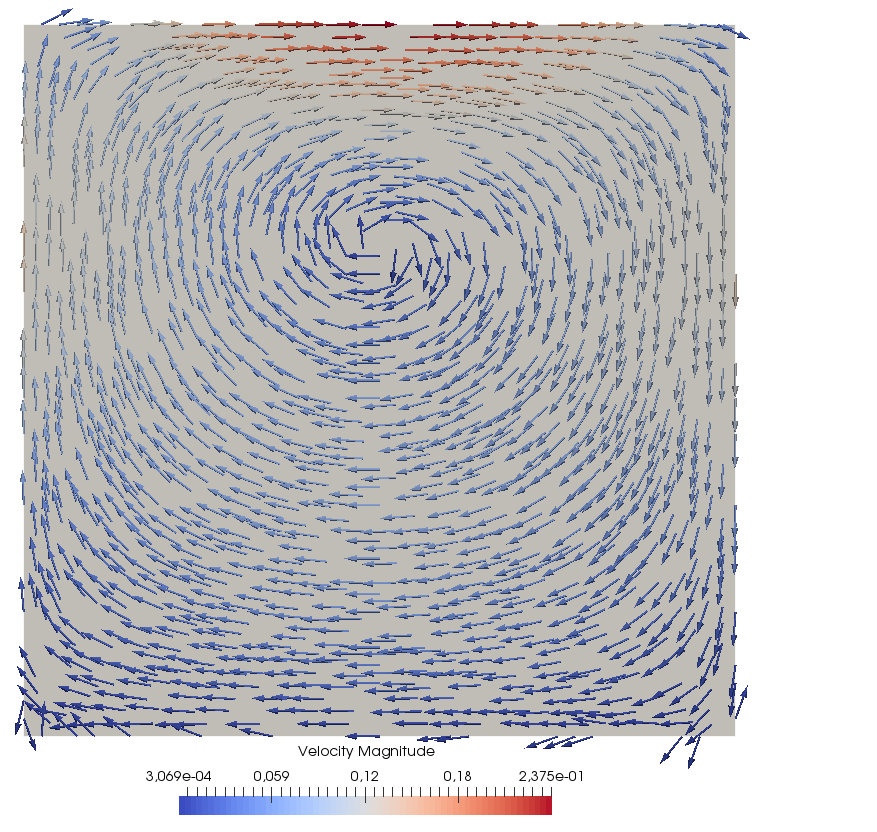
\includegraphics[
    width=\graphHratio\linewidth,
    height=\graphVratio\linewidth
    ]{img/v-eps0}
    &
    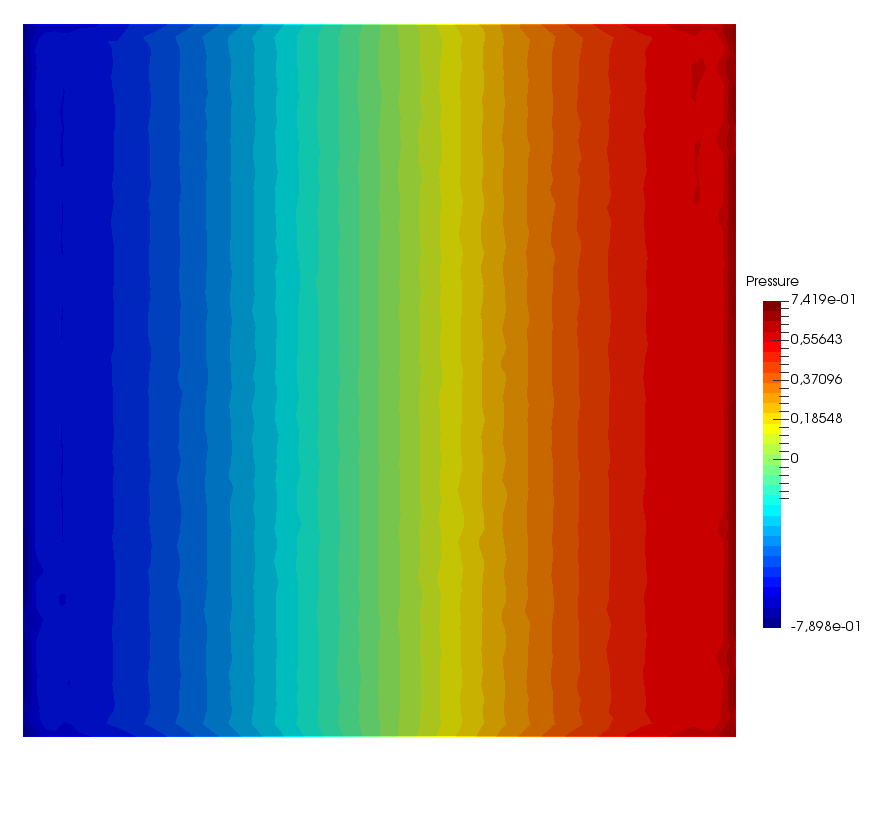
\includegraphics[
    width=\graphHratio\linewidth,
    height=\graphVratio\linewidth
    ]{img/p-eps0}
  \end{tabular}
  \\[1em]
  \textbf{Figure 2.} DG Non-Hydrostatic Cavity test ($\varepsilon=10^{-8}$).
\end{center}

\end{frame}

\section{Application to Non-Hydrostatic Large-Scale Boussinesq Equations}

\subsection{Extension of Previous Techniques to Boussinesq Equations}
%----------------------------------------------------------------------
\newcommand{\frametitlestep}[3]{\frametitle{%
\textit{\bfseries Step #2}\hskip0.5em #3 \hfill #1~\mbox{}}}

\begin{frame}{Euler method}
\begin{small}
  \begin{block}{}\vspace{-1em}
    \begin{align*}
      \dt \uu + \uu\cdot\gradx\uu + \vv\,\dz\uu  - \Delta_\visc\uu
      + \frac 1 \rho_\star \gradx \pp=
      \\
      \varepsilon^2 \Big( \dt \vv + \uu\cdot\gradx\vv +
          \vv\,\dz\vv - \Delta_\visc\vv \Big)
        \displaystyle
        + \frac 1 \rho_\star \dz \pp +
        \frac{
          \rho\,\gravity}{\rho_\star} =
        0\hskip+0.5em
      \\
      \div\uu + \dz\vv = 0\hskip+0.5em
    \end{align*}
  \end{block}
  \begin{block}{}\vspace{-1em}
    \begin{align*}
      \dt \Te  + (\uu \cdot \gradx) \Te + (\vv\cdot\dz) \Te  - \nu_\Te\Delta \Te &= \fT
      \\[0.3em]
      \dt \Sa  + (\uu \cdot \gradx) \Sa + (\vv\cdot\dz) \Sa -
      \nu_\Sa\Delta \Sa &= \fS
      \\[0.3em]
      \rho = \rho_\star\big(1-\beta_\Te(\Te-\Te_\star) + \beta_\Sa(\Sa&-\Sa_\star)\big)
    \end{align*}
  \end{block}
  \textbf{Euler} semi-implicit scheme:
    \begin{itemize}\itemsep0.66em
    \item \textbf{Step 1}. Calculate \alert{temperature}, \alert{salinity} and then
      \alert{density} (decoupling from momentum equations)
    \item \textbf{Step 2}. Use density to obtain \alert{velocity} and
      \alert{pressure} (solve \underline{\structure{Anisotropic Navier-Stokes using previous techniques}})
    \end{itemize}
\end{small}
\end{frame}

\begin{frame}{Cavity test + temperature}
  \begin{itemize}
  \item $\varepsilon=0$, \FEthreeSpacesP221 elements, ``random''
    unstructured mesh
  \item Flow: \textbf{wind traction} on surface (left to right)
  \item Temperature: \textbf{heat transfer from surface}
  \end{itemize}
%  \pause
  \begin{center}
    \PlayVideoWithLabel[0.45\linewidth][0.45\linewidth][Streamlines]{%
      video/euler-square-streamlines.avi}
    \hfill
    \PlayVideoWithLabel[0.45\linewidth][0.45\linewidth][Temperature]{%
      video/euler-square-temperature.avi}
  \end{center}
\end{frame}

\begin{frame}{Gibraltar strait 2D flow + temperature + salinity}
  \vskip0.3em
  \begin{columns}
    \column{0.6\linewidth}
    \PlayVideoWithLabel[0.9\linewidth][0.9\linewidth][Streamlines]{%
      video/euler-gibraltar-streamlines.avi}
    \column{0.37\linewidth}
    \PlayVideoWithLabel[0.89\linewidth][0.88\linewidth][Salinity]{%
      video/euler-gibraltar-salinity.avi}
    \par\vskip-0.6em
    \PlayVideoWithLabel[0.89\linewidth][0.88\linewidth][Temperature]{%
      video/chapter4/euler-gibraltar-temperature.avi}
    \end{columns}
  \end{frame}

%% ,---------------------------------------------------------------------
%% | Conclusions and future work
%% `---------------------------------------------------------------------
\begin{frame}{Conclusions}
  \large
  \begin{itemize}\itemsep1.3em
  \item \alert{\textbf{Unified framework}} for approximation of \textbf{Non-Hydrostatic Navier-Stokes}
    and \textbf{Primitive Equations} of the Ocean
  \item Idea:  \alert{stabilizing vertical
      velocity} makes possible:\bigskip
    \begin{itemize}\itemsep0.5em
    \item \normalsize The use of \alert{standard FE tools and techniques}
    \item \normalsize With optimal (Stokes-like) error orders.
    \end{itemize}
  \item Also exploring \structure{Discontinuous Galerkin} approximations
  \item Straightforward \alert{extension to Boussinesq} (variable density) equations
    % like mesh adaptation
    % can be used, in \alert{more general meshes} than previous schemes
  \end{itemize}
\end{frame}

% \begin{frame}{Some possible extensions}
%   Previous schemes open a path for future improvement:
    %   % Some interesting tasks are still pending, including:
    %   \bigskip
    %   \begin{enumerate}\itemsep0.6em
    %   \item \alert{\textbf{Test with realistic physical data}} \exclamation
    %   \item Publish results on \alert{variable density} and \alert{time-stepping} methods
    %   \item ...
    %   \end{enumerate}
    % \end{frame}

    \SetEmptyBackground
    \begin{frame}

      \begin{flushright}
        \Huge\it
        Thank

        you!
      \end{flushright}
    \end{frame}
    \SetDefaultBackground

    %% ,-------------
    %% | Bibliography
    %% `-------------

    \setbeamertemplate{footline}[default]

    \begin{frame}[allowframebreaks]{Bibliography}
      \bibliographystyle{alpha}
      \bibliography{biblio-short.bib}
    \end{frame}

    \appendix

    \begin{frame}{Credits}
      \begin{itemize}
      \item Icon
      \href{https://commons.wikimedia.org/wiki/File:Ampoule-electrique.png}{Ampoule-electrique.png} from Wikimedia Commons, the free media repository.
    \end{itemize}
    \end{frame}
  \end{document}


  %%% Local Variables:
  %%% coding: utf-8
  %%% TeX-master: t
  %%% mode: latex
  %%% ispell-local-dictionary: "english"
  %%% End:
